\documentclass[10pt,a4paper]{article}
\usepackage[margin=2.2cm]{geometry}
\usepackage[T1]{fontenc}
\usepackage[utf8]{inputenc}


\usepackage{amsmath}
\usepackage{amssymb}
\usepackage{mathptmx}
\usepackage{booktabs}
\usepackage{graphicx}
\usepackage{xcolor}
\usepackage{caption}
\usepackage{subcaption}
\usepackage{listings}
\usepackage{float}
\usepackage{textcomp}
\usepackage[hidelinks]{hyperref}
\usepackage{xurl}
\captionsetup{font=small,labelfont=bf}
% Layout: never leave a single line of a paragraph alone at the top or bottom of a page
\widowpenalty=10000
\clubpenalty=10000
\displaywidowpenalty=10000
\interlinepenalty=10000
\raggedbottom
\emergencystretch=3em
\lstset{basicstyle=\ttfamily\footnotesize,columns=fullflexible,frame=single,
        framerule=0.3pt,rulecolor=\color{gray},xleftmargin=2pt,xrightmargin=2pt}
\graphicspath{{../figures/}}
\makeatletter\newcommand{\tabinput}[1]{\@@input #1 }\makeatother

% ---------------------------------------------------------------
% EDIT HERE: link to your GitHub repository (mandatory)
\newcommand{\repourl}{https://github.com/aimarsantana/BigData-Assignment01-MatMul}
% ---------------------------------------------------------------

\title{\textbf{How Matrix Size Drives Runtime and Memory of a Basic\\
Triple-Loop Matrix Multiplication in Python, Java and C}\\[4pt]
\large Big Data -- Individual Assignment 1: Basic Matrix Multiplication in Different Languages}
\author{Aimar Daniel Alejandro Santana\\
Grado en Ciencia e Ingeniería de Datos, Universidad de Las Palmas de Gran Canaria\\
\small Repository: \url{\repourl}}
\date{October 2026}

\begin{document}
\maketitle

%==============================================================
\begin{abstract}
We measure how the matrix size $n$ affects the runtime and the peak memory of one and the
same basic $O(n^3)$ triple-loop (i-j-k) dense matrix multiplication written in C, Java and
Python. The three versions read identical binary64 input files and produce bit-identical
results. They were timed on the same 2-vCPU Intel Xeon virtual machine, with only the kernel
inside the timer, 5--10 repetitions per configuration (median and IQR reported), and a declared
budget of 200\,s per multiplication. Every language grows at least cubically, but the cost per
inner iteration is not constant. It rises with $n$, by up to $\approx 8\times$ for C, $\approx 14\times$ for Java and
$\approx 2.5\times$ for Python, because the stride-$n$ column access to $B$ steps out of the
caches. C and Java stay within a factor of $\approx 0.7$--$2.6$ of each other. Neither is
uniformly faster: Java is ahead at $n=512$ and $768$, and C at $n\ge1024$. CPython is
$41$--$104\times$ slower than C. The largest feasible sizes are $n=2048$ for Java,
$n=1536$ for C (its $n=2048$ run exceeded the budget in the main experiment but took 108\,s in a
separate probe) and $n=1024$ for Python. Peak memory grows as $n^2$ on top of a fixed runtime
cost of about 2\,MiB (C), 41\,MiB (Java) and 11\,MiB (Python). These conclusions apply only to
the tested implementations, settings and machine.
\end{abstract}

%==============================================================
\section{Introduction and objective}
Dense matrix multiplication is the reference kernel of numerical computing and a natural
starting point for a course on scalable data processing: it is simple to state, its
arithmetic cost is known exactly, and its performance depends strongly on how the
implementation interacts with the processor and the memory hierarchy. Before optimised,
sparse, parallel and distributed variants are studied in later assignments, this study
establishes a validated, reproducible \emph{baseline} for the same basic algorithm in three
languages with very different execution models: an ahead-of-time compiled language (C), a
JIT-compiled managed language (Java) and an interpreted dynamic language (CPython).

\paragraph{Research question.} \emph{How does the matrix size $n$ affect the runtime and the
peak memory of the same basic $O(n^3)$ triple-loop multiplication implemented in Python,
Java and C, when inputs, algorithm, loop order, numeric type, timing boundary and machine are
held fixed?}

\paragraph{Factor, outcomes and comparison.} The factor varied is $n$ (side of an
$n\times n$ matrix); the categorical factor is the implementation language. The outcomes are
(i) time per multiplication of the kernel and (ii) peak resident memory of the process.

\paragraph{Hypotheses (predictions, stated before running the experiments).}
\begin{enumerate}
\item[H1] Runtime grows approximately as $n^3$ in all three languages, but the constant per
inner iteration is not constant: it should increase for large $n$ because the column-wise
access to $B$ stops fitting in cache.
\item[H2] C and Java (after JIT warm-up) are within a small factor of each other, while
CPython is one to two orders of magnitude slower because each multiply-add is executed by the
bytecode interpreter on boxed float objects.
\item[H3] Peak memory grows as $n^2$; Java adds a large fixed runtime cost, and Python needs
several times more bytes per element than the 8 bytes of a raw \texttt{double}.
\end{enumerate}

%==============================================================
\section{Background}
\paragraph{Algorithm.} For $C=AB$ with $A,B\in\mathbb{R}^{n\times n}$, the definition
$c_{ij}=\sum_{k=0}^{n-1} a_{ik}b_{kj}$ gives the classical triple loop with exactly $n^3$
multiplications and $n^3$ additions ($2n^3$ floating-point operations) \cite{golub2013}.
The six loop orders perform the same arithmetic but access memory differently. In the
\emph{i-j-k} order used here, the innermost loop reads row $i$ of $A$ contiguously
(stride 1) and column $j$ of $B$ with stride $n$ elements, which defeats spatial locality and
makes the kernel memory-bound once $B$ no longer fits in the caches
\cite{drepper2007,hennessy2017}. When the stride is a large power of two, consecutive elements
of a column map to a few cache sets and evict each other (conflict misses) \cite{lam1991}.

\paragraph{Execution models.} C is compiled ahead of time to machine code. Java bytecode is
first interpreted and then compiled by the HotSpot JIT compiler once methods or loops become
hot, so early executions are slower and warm-up runs must be separated from measured runs
\cite{georges2007}. CPython interprets bytecode; every \texttt{float} is a heap object
(24 bytes on 64-bit CPython, measured with \texttt{sys.getsizeof}) referenced by an 8-byte
pointer from its list, and every arithmetic operation involves type dispatch and the
allocation of a new result object \cite{pythondatamodel}.

\paragraph{Floating-point accuracy.} A length-$n$ dot product in binary64 satisfies
$|\hat c_{ij}-c_{ij}|\le\gamma_n\,(|A||B|)_{ij}$ with $\gamma_n=nu/(1-nu)$ and $u=2^{-53}$
\cite{higham2002}. This bound is used as the tolerance for validation. Since Java~17 all
floating-point arithmetic is strict IEEE~754 \cite{jep306}; with GCC \texttt{-O2} on the
baseline x86-64 target no fused multiply-add is emitted and no reassociation is allowed
(no \texttt{-ffast-math}); CPython performs one IEEE operation per bytecode. The three kernels
therefore execute the same sequence of rounded operations, which makes a bitwise comparison
of their outputs a strong correctness check.

\paragraph{Benchmark reporting.} Following common recommendations for performance studies
\cite{hoefler2015,georges2007}, we keep every raw sample, summarise with the median and the
interquartile range (IQR), report the number of repetitions, and describe the timer boundary.

%==============================================================
\section{Methodology}
\subsection{Implementations and storage layouts}
All three programs implement the same kernel, with the same loop order (i-j-k), the same
local scalar accumulator and the same numeric type (IEEE~754 binary64):
\begin{lstlisting}
for i in 0..n-1:  for j in 0..n-1:
    s = 0.0
    for k in 0..n-1:  s += A[i][k] * B[k][j]
    C[i][j] = s
\end{lstlisting}
No library call replaces the loops. Unavoidable language-specific differences are the
storage layouts (Table~\ref{tab:impl}). Source files: \texttt{src/c/matmul.c},
\texttt{src/java/MatMul.java}, \texttt{src/python/matmul.py}.

\begin{table}[H]
\centering\small
\caption{Implementations and fixed settings.}\label{tab:impl}
\begin{tabular}{p{1.4cm}p{5.6cm}p{8.0cm}}
\toprule
Language & Storage layout & Toolchain and fixed settings \\
\midrule
C & One contiguous row-major block of $n^2$ \texttt{double} per matrix plus an array of $n$ row
pointers (\texttt{A[i][k]} syntax). & GCC 13.3.0, \texttt{gcc -O2 -std=c11 -Wall -Wextra}
(no \texttt{-march}, no \texttt{-ffast-math}). \\
Java & \texttt{double[][]}: each row is a separate contiguous \texttt{double[]} heap object
(16-byte header); rows are not guaranteed to be adjacent. & OpenJDK 21.0.12 HotSpot Server VM,
\texttt{javac --release 21}; \texttt{java -Xms64m -Xmx4g -XX:+UseSerialGC}; default tiered JIT;
3 warm-up runs in the same JVM. \\
Python & List of lists; each element is a boxed \texttt{float} object (24\,B) referenced by an
8\,B pointer. & CPython 3.13.16 (no JIT enabled, standard GIL build); pure-Python loops; NumPy
not used in the kernel; 1 warm-up run. \\
\bottomrule
\end{tabular}
\end{table}

\subsection{Inputs}
All implementations read the \emph{same} binary files, so the logical inputs are identical
across languages. The matrices are generated once by \texttt{scripts/generate\_inputs.py}
with NumPy's PCG64 generator \cite{oneill2014} (seed 20261012 for $A$, 20261013 for $B$),
uniformly distributed in $[-1,1)$, stored as raw little-endian row-major binary64. A
manifest with the SHA-256 hash of every file is saved with the data.

\subsection{Environment}
\begin{table}[H]
\centering\small
\caption{Execution environment (full output of \texttt{scripts/collect\_environment.sh} in
\texttt{results/environment.txt}).}\label{tab:env}
\begin{tabular}{ll}
\toprule
CPU & Intel Xeon Processor @ 2.80\,GHz (Cascade Lake family 6 model 85, AVX-512 capable), KVM guest \\
Cores / logical CPUs & 2 vCPUs: 1 socket, 2 cores, 1 thread per core; no affinity pinning \\
Caches (as reported) & L1d 32\,KiB/core, L2 1\,MiB/core, L3 33\,MiB shared \\
RAM & 7.8\,GiB (8\,421\,236\,736 bytes), no swap; transparent huge pages: \texttt{madvise} \\
OS & Ubuntu 24.04.5 LTS, Linux 6.18 (cloud virtual machine, shared physical host) \\
Software & gcc 13.3.0; OpenJDK 21.0.12 (HotSpot); CPython 3.13.16; NumPy 2.5.3 (inputs/reference only) \\
Threads & All kernels single-threaded; JVM internal threads (JIT, 1 serial GC thread) not controlled \\
\bottomrule
\end{tabular}
\end{table}
Because the machine is a virtual machine on a shared host, other tenants can disturb caches and
CPU time. Every configuration is measured on the same machine, so the comparison between
languages is controlled. Absolute times, however, apply only to this environment.

\subsection{Correctness checks}
Before benchmarking, \texttt{tests/validate.py} runs every implementation on: a hand-computed
$2\times2$ and $3\times3$ product, $IR=R$, $RI=R$, $0R=0$, $n=1$ (all required to be
\emph{exactly} equal), and random matrices with $n\in\{7,33,100,256\}$, compared against NumPy
(used only as a reference, not as an implementation) with the componentwise tolerance
$|C-C_{\text{ref}}|\le 2\gamma_n(|A||B|)$; the factor 2 accounts for the rounding error of the
reference itself. In addition the outputs of the three languages are compared for
\emph{bitwise} equality. During every benchmark run a checksum of $C$ is computed after the
timer is stopped, so the result is always consumed and cannot be optimised away.

\subsection{Measurement protocol}
\begin{itemize}
\item \textbf{Timer boundary: kernel only.} Input loading and allocation/zeroing of $C$ happen
before the timer starts; the checksum is computed after it stops. Monotonic timers:
\texttt{clock\_gettime(CLOCK\_MONOTONIC)} (C), \texttt{System.nanoTime()} (Java),
\texttt{time.perf\_counter\_ns()} (Python).
\item \textbf{Sizes:} $n\in\{64,128,256,384,512,768,1024,1536,2048\}$ (powers of two plus
intermediate values to expose trends).
\item \textbf{Repetitions:} one fresh process per (language, $n$); 10 measured samples for
$n\le512$ and 5 for $n>512$ (justified by cost: one Python run at $n=1024$ takes about
2.5~minutes). Warm-up runs, recorded but excluded: C 1, Java 3, Python 1. For $n=64$ and
$n=128$ each sample times a batch of 20 and 5 consecutive multiplications respectively and the
time per multiplication is reported.
\item \textbf{Budgets (declared in advance):} at most 200\,s per single multiplication and 4\,GB
peak RSS. If a configuration exceeds the budget it is killed, recorded as \textsc{timeout},
and larger sizes for that language are not attempted.
\item \textbf{Memory metric:} peak resident set size of the benchmark process (\texttt{VmHWM}),
read by each program from \texttt{/proc/self/status} just before exiting
\cite{proc5}. It includes the runtime (interpreter/JVM), the three matrices and any
temporaries; it is \emph{not} the size of the arrays alone. A baseline run per language that
loads the $n=64$ inputs but performs no multiplication measures the fixed runtime cost. We
also report the analytical raw array size $3\cdot8n^2$ bytes. For Java the JVM's own heap
statistics are logged but are a different quantity and are not compared with RSS.
\item \textbf{Execution order and noise:} configurations run sequentially (increasing $n$;
C, Java, Python) with no other user workload. The kernels are single-threaded; the JVM still
runs internal threads (JIT compiler, one serial GC thread), which may use the second vCPU.
\item \textbf{Summary statistics:} median and IQR (with min/max) of measured samples; every raw
sample is kept in \texttt{results/raw\_samples.csv}.
\end{itemize}

%==============================================================
\clearpage
\section{Results}
\subsection{Correctness}
All 40 checks passed (\texttt{results/validation.csv}). The six exact cases gave exactly the
expected matrices in all three languages. In the random cases the largest error with respect to
NumPy was $1.1\times10^{-14}$ at $n=256$, which is at most 9\,\% of the allowed bound
$2\gamma_n(|A||B|)$. The outputs of C, Java and Python were \emph{bitwise identical} in every
case. This confirms that the three kernels perform the same sequence of IEEE operations. It also
means that differences in runtime cannot come from differences in arithmetic.

\subsection{Runtime}
Table~\ref{tab:time} reports every configuration and Figure~\ref{fig:runtime} plots the medians
on log--log axes. All configurations completed within the budget except
Python at $n=1536$ and C at $n=2048$, which exceeded 200\,s in the first (warm-up) run.
Following the stop rule, Python at $n=2048$ was not attempted. The largest tested feasible sizes
are therefore $n=2048$ (Java), $n=1536$ (C) and $n=1024$ (Python). The largest attempted size
was $2048$ for C and Java and $1536$ for Python. Relative variability was mostly below 12\,\% of
the median. The exception is Python at $n=256$ (20\,\%), which we attribute to interference on
the shared host.

\begin{table}[H]
\centering\footnotesize
\caption{Time per multiplication (kernel only). Reps = measured samples (warm-up excluded);
``$\times b$'' = each sample timed $b$ consecutive multiplications. IQR is also given as a
percentage of the median. ns/iter = median$/n^3$. MFLOP/s = $2n^3$/median.}\label{tab:time}
\begin{tabular}{lrlllllrr}
\toprule
Language & $n$ & Reps & Median & IQR (\% of median) & Min & Max & ns/iter & MFLOP/s \\
\midrule
\tabinput{generated/table_time.tex}
\bottomrule
\end{tabular}
\end{table}

\begin{figure}[H]
\centering
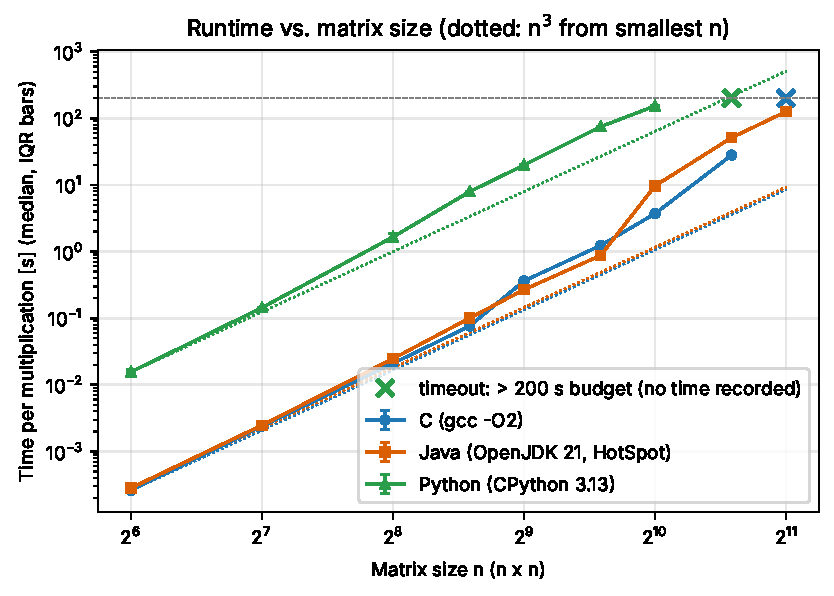
\includegraphics[width=0.78\linewidth]{fig_runtime_loglog.pdf}
\caption{Median time per multiplication against $n$ (log--log). Error bars show the IQR (mostly
smaller than the markers). Dotted lines extrapolate an exact $n^3$ law from the smallest size of
each language. Crosses mark configurations killed at the 200\,s budget.}\label{fig:runtime}
\end{figure}

\paragraph{Growth versus the cubic model.} Table~\ref{tab:fit} fits $\log t = a + b\log n$ for
$n\ge256$. Python grows close to cubically ($b=3.27$). C ($b=3.97$) and Java ($b=4.29$) grow
clearly faster than $n^3$ over the sizes tested. Figure~\ref{fig:iter} explains why: if growth
were exactly cubic, the time per inner iteration (median$/n^3$) would be flat. Instead it
increases in steps. For C it goes from 1.0\,ns ($n=64$) to 2.7\,ns ($n=512$--$768$), 3.5\,ns
($n=1024$) and 7.7\,ns ($n=1536$). Java follows a similar path but jumps between $n=768$
(1.9\,ns) and $n=1024$ (9.0\,ns), reaching 14.7\,ns at $n=2048$. Python rises from 59\,ns to
140--165\,ns.

\begin{table}[H]
\centering\small
\caption{Least-squares slope of $\log(\text{median time})$ against $\log n$ for $n\ge256$
(slope 3 = cubic).}\label{tab:fit}
\begin{tabular}{lrrrr}
\toprule
Language & Sizes & Points & Slope $b$ & $R^2$ \\
\midrule
\tabinput{generated/table_fit.tex}
\bottomrule
\end{tabular}
\end{table}

\begin{figure}[H]
\centering
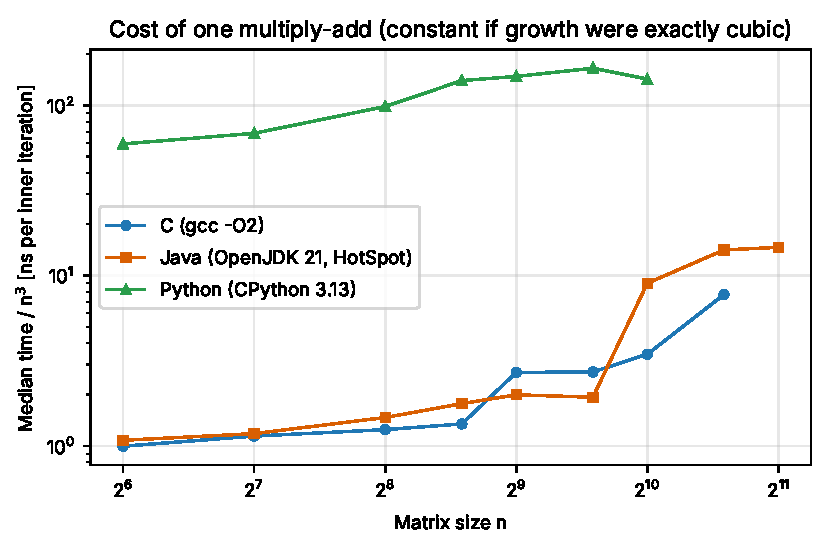
\includegraphics[width=0.72\linewidth]{fig_time_per_iteration.pdf}
\caption{Median time divided by $n^3$: the cost of one multiply-add of the inner loop.}\label{fig:iter}
\end{figure}

\paragraph{Relative performance.} Table~\ref{tab:ratio} and Figure~\ref{fig:ratio} give the
ratio of medians with respect to C. Java is within 8--32\,\% of C for $n\le384$ and faster than
C at $n=512$ and $768$ (ratio 0.74 and 0.71). It is $2.6\times$ and $1.8\times$ slower at
$n=1024$ and $1536$. Python is $41$--$104\times$ slower than C.

\begin{table}[H]
\centering\small
\begin{minipage}{0.36\linewidth}\centering
\caption{Median time ratios.}\label{tab:ratio}
\begin{tabular}{rrr}
\toprule
$n$ & Java/C & Python/C \\
\midrule
\tabinput{generated/table_ratio.tex}
\bottomrule
\end{tabular}
\end{minipage}\hfill
\begin{minipage}{0.6\linewidth}\centering
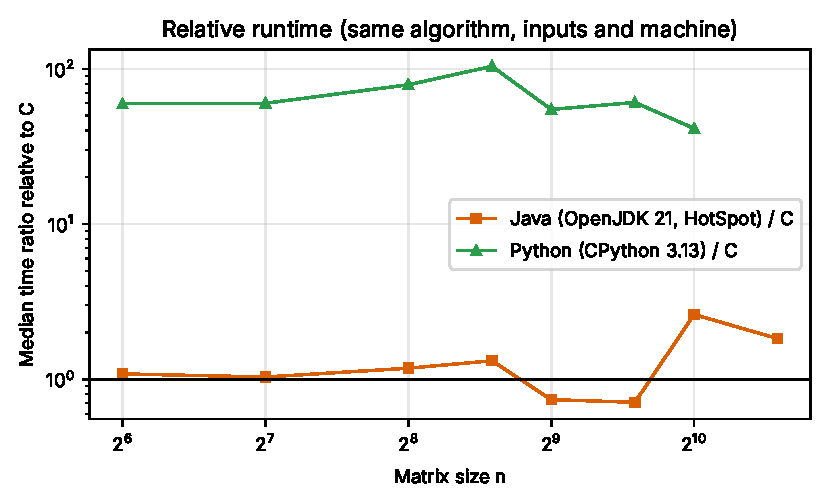
\includegraphics[width=\linewidth]{fig_ratio_to_c.pdf}
\captionof{figure}{Ratios of median time relative to C.}\label{fig:ratio}
\end{minipage}
\end{table}

\paragraph{Java warm-up.} Figure~\ref{fig:warmup} shows each run inside one JVM, divided by the
median of the measured runs. The first execution at $n=128$ (a batch of five multiplications)
takes $1.7\times$ the steady-state time, because the code is still interpreted or only partly
compiled. From the second run onwards the times fall within normal noise. Three warm-up runs are
therefore enough, and excluding them avoids biasing Java's results.

\begin{figure}[H]
\centering
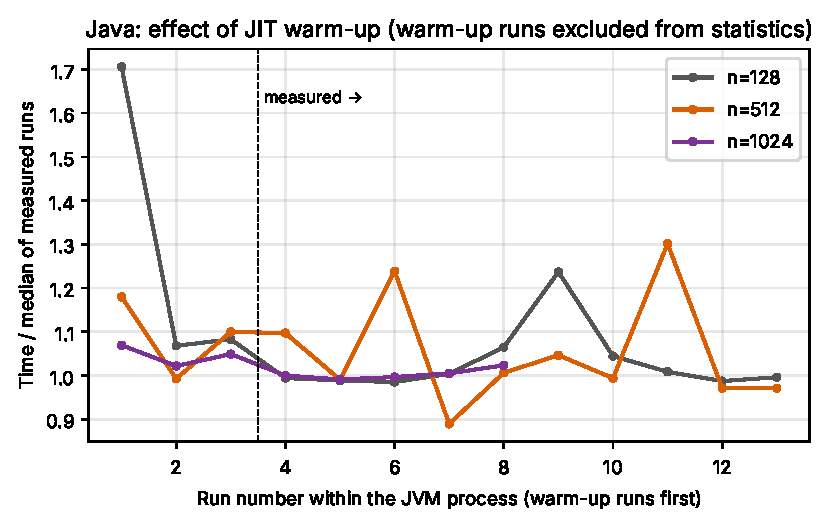
\includegraphics[width=0.72\linewidth]{fig_java_warmup.pdf}
\caption{Java: time of every run inside one JVM process divided by the median of the measured
runs. The first three runs are warm-up and are excluded from the statistics.}\label{fig:warmup}
\end{figure}

\subsection{Memory}
Table~\ref{tab:mem} and Figure~\ref{fig:mem} report peak RSS (VmHWM). The baseline row shows the
fixed cost of each runtime after loading the $n=64$ inputs without multiplying. The cost on top
of that baseline grows as $n^2$:
\begin{itemize}
\item \textbf{C}: peak RSS is close to the raw array size plus 1.7\,MiB
(e.g.\ 25.7\,MiB against 24.0\,MiB of arrays at $n=1024$).
\item \textbf{Java}: about 41\,MiB of fixed JVM cost plus heap. At $n=2048$ the 205\,MiB includes
the 96\,MiB of arrays, the 32\,MiB transient \texttt{byte[]} used when reading each input file,
and the space the garbage-collected heap has committed but not yet released.
\item \textbf{Python}: grows fastest. At $n=1024$ the 131\,MiB is about $5.5\times$ the raw
arrays. Subtracting the baseline gives $\approx40$ bytes per element. This matches a 24-byte
\texttt{float} object plus an 8-byte list pointer per element, plus list headers and the
transient \texttt{array} buffer used while loading the inputs.
\end{itemize}
These numbers measure different things (process RSS, not live data), so they should be read as
the memory footprint of each program, not as the size of the matrices.

\begin{table}[H]
\centering\small
\begin{minipage}{0.44\linewidth}\centering
\caption{Peak RSS [MiB] and raw array size $3\cdot8n^2$ bytes [MiB].}\label{tab:mem}
\setlength{\tabcolsep}{4pt}
\begin{tabular}{rrrrr}
\toprule
$n$ & Arrays & C & Java & Python \\
\midrule
\tabinput{generated/table_memory.tex}
\bottomrule
\end{tabular}
\end{minipage}\hfill
\begin{minipage}{0.53\linewidth}\centering
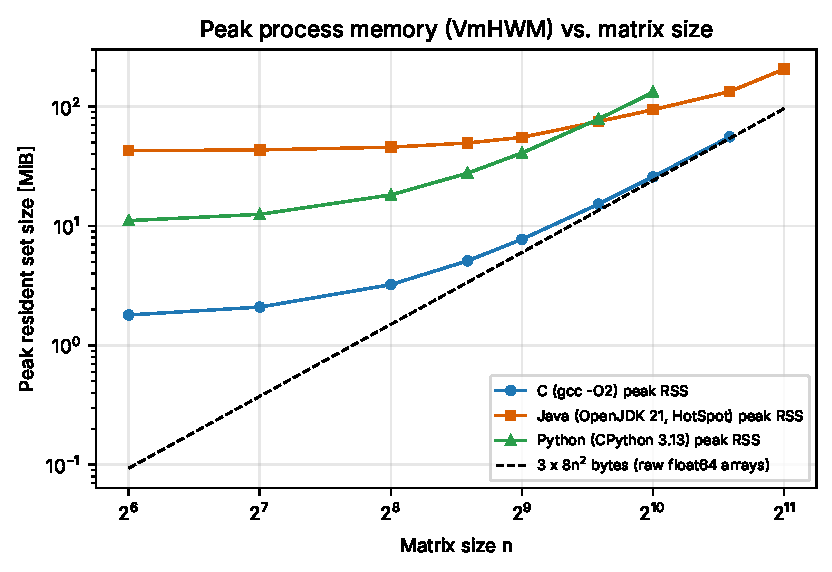
\includegraphics[width=\linewidth]{fig_memory.pdf}
\captionof{figure}{Peak RSS against $n$ (log--log); the dashed line is the raw size of the three
float64 arrays.}\label{fig:mem}
\end{minipage}
\end{table}

\subsection{Supplementary experiments (separate from the controlled comparison)}
Two unexpected observations from the main study were examined with additional runs. These used
the same kernel, flags, input generator and timer boundary, under their own declared settings
(\texttt{config/supplementary\_*.json}).

\paragraph{A. Sizes around powers of two.} C shows a sharp step at $n=512$ that Java does not.
We therefore measured $n\in\{500,511,512,513,1000,1023,1024,1025\}$ (Table~\ref{tab:supp},
Figure~\ref{fig:supp}). For C, $n=512$ costs 2.76\,ns per iteration, compared with 1.47--1.53\,ns
at 500, 511 and 513. Java shows no such step (1.82--1.94\,ns). Around $n=1000$ there is no
power-of-two effect in either language: all C sizes lie at 3.4--4.9\,ns and all Java sizes at
9.4--10.1\,ns.

\begin{table}[H]
\centering\small
\begin{minipage}{0.32\linewidth}\centering
\caption{Supplementary A: median ns per inner iteration.}\label{tab:supp}
\begin{tabular}{rrr}
\toprule
$n$ & C & Java \\
\midrule
\tabinput{generated/table_supp.tex}
\bottomrule
\end{tabular}
\end{minipage}\hfill
\begin{minipage}{0.64\linewidth}\centering
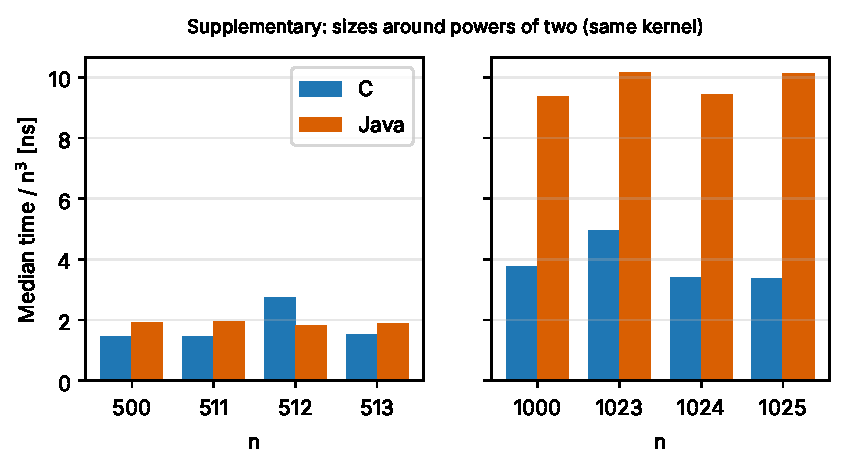
\includegraphics[width=\linewidth]{fig_supp_alignment.pdf}
\captionof{figure}{Supplementary A: cost per inner iteration at and around powers of two.}\label{fig:supp}
\end{minipage}
\end{table}

\paragraph{B. The C time-out at $n=2048$.} Fresh processes for $n=2047$ and $n=2048$ were run
with an extended 900\,s budget and 3 measured runs (Table~\ref{tab:supplarge}). In this probe C
completed $n=2048$ in a median of 107.6\,s, well inside the original budget. In the main run it
had not finished a single multiplication in 200\,s. C at $n=2047$ took 95.3\,s. Java took
$\approx130$\,s at both sizes, close to its main-study value (125.8\,s). The main-study time-out
is kept as a result. It shows that the time of one C process at $n=2048$ can vary by more than a
factor of two between processes. Within each process the runs were very stable.

\begin{table}[H]
\centering\small
\caption{Supplementary B: extended-budget probe (900\,s), 3 measured runs per configuration.}\label{tab:supplarge}
\begin{tabular}{lrrrrr}
\toprule
Language & $n$ & Reps & Median [s] & Range [s] & ns/iter \\
\midrule
\tabinput{generated/table_supp_large.tex}
\bottomrule
\end{tabular}
\end{table}

%==============================================================
\section{Discussion}
\paragraph{Answer to the research question.} On this machine, runtime grows with $n$ at least
as fast as the cubic operation count for all three implementations (H1 confirmed). Peak memory
grows as $n^2$ above a language-specific fixed cost (H3 confirmed). Between languages, the gap
is large and stable for Python ($\approx40$--$100\times$ slower than C). For C and Java the
relation depends on $n$: neither is faster at every size, so H2 holds only in part.

\paragraph{Interpreter effects (Python).} With bitwise-identical arithmetic, Python's cost of
59--165\,ns per inner iteration, against 1--8\,ns in C, comes from executing the inner loop as
bytecode. Each \texttt{s += A[i][k]*B[k][j]} performs several list subscriptions, dynamic type
checks and the allocation of new \texttt{float} objects \cite{pythondatamodel}. This
per-operation overhead is so large that memory effects matter less, which is why Python's growth
exponent (3.27) is the closest to the cubic model. Its per-iteration cost still rises by
$\approx2.5\times$ between $n=64$ and $n=768$. A plausible explanation is that the boxed
\texttt{float} objects of a column of $B$ are scattered in memory, so they stop fitting in cache.
We did not measure cache misses, so this remains a hypothesis.

\paragraph{Runtime effects (Java).} After warm-up, HotSpot's JIT-compiled loop is competitive
with \texttt{gcc -O2} for $n\le768$, as long as the working set stays in cache. Excluding the
warm-up runs was essential: including them would add up to 70\,\% to the first sample at
$n=128$ \cite{georges2007}. The JVM also has the largest fixed memory cost.

\paragraph{Memory-layout effects (C and Java).} In i-j-k order the inner loop walks down a column
of $B$ with a stride of $8n$ bytes. A cache line brings in $B[k][j..j+7]$, so lines can be reused
by the next seven values of $j$, but only if the $n$ lines of a column stay in cache. As $n$
grows, the column and then all of $B$ stop fitting in L1, L2 and L3. Each level that is exceeded
raises the cost per iteration \cite{drepper2007,hennessy2017}. This produces the steps in
Figure~\ref{fig:iter} and the slopes above 3. Supplementary experiment A supports a
memory-layout explanation for one specific step. In C every row of $B$ starts exactly $8n$ bytes
after the previous one. At $n=512$ this is 4096\,bytes, so all elements of a column map to the
same L1 cache set and evict each other (conflict misses) \cite{lam1991}. Neighbouring sizes
(511, 513) do not show the step. In Java each row is a separate array with a 16-byte header, so
consecutive rows are not exactly a power of two apart. Java shows no step at 512, which is why it
beats C there. Above $n\approx1000$, Java pays more per iteration than C (9--15\,ns against
3.4--4.9\,ns at $n\approx1000$). This is not a power-of-two effect (supplementary A). Candidate
explanations include:
\begin{itemize}
\item the extra instructions per iteration (row-reference load, bounds check), which reduce the
number of cache misses the CPU can overlap;
\item address-translation (TLB) misses, because at this size each access to $B$ touches a
different 4\,KiB page;
\item the heap placement of the row arrays.
\end{itemize}
Hardware performance counters are not available in this virtual machine, so we cannot decide
between them. This question remains open.

\paragraph{Limitations.}
\begin{itemize}
\item The machine is a 2-vCPU cloud virtual machine on a shared host. Absolute times, and in
particular the C $n=2048$ result (time-out in one process, 108\,s in another), may be affected by
other tenants and by the physical pages the operating system assigns. We could not separate these
causes.
\item No performance counters were available, so the explanations based on caches and the TLB are
hypotheses consistent with the data, not measurements.
\item Large sizes use only 5 repetitions (3 in the probe) because of their cost. Each
configuration runs in one process, so variation between processes is captured only by the
supplementary probe.
\item Only one compiler level (\texttt{-O2}), one JVM configuration and one Python implementation
were tested. Other settings (e.g.\ \texttt{-O3 -march=native}, PyPy, another loop order) are
language-specific optimisations outside this controlled baseline.
\item Peak RSS includes transient buffers used to load the inputs and, for Java, heap space that
is committed but not live. It measures each program's footprint, not the matrices alone.
\end{itemize}

%==============================================================
\section{Conclusions}
Within the tested scope (one 2-vCPU Intel Xeon VM; gcc 13.3 \texttt{-O2}, OpenJDK 21
HotSpot after 3 warm-up runs, CPython 3.13; float64 inputs uniform in $[-1,1)$; kernel-only
timing), this study establishes four findings:
\begin{enumerate}
\item The three straightforward triple-loop implementations are correct and produce
bit-identical results.
\item Their runtime grows at least cubically with $n$. Beyond the $n^3$ operation count, the
memory hierarchy adds a cost per iteration that grows with $n$: up to $\approx8\times$ in C,
$\approx14\times$ in Java and $\approx2.5\times$ in Python between the smallest and largest
feasible sizes.
\item CPython is about 40--100 times slower than C. C and Java are close for small sizes, and
which one is faster depends on $n$ and on the memory layout (power-of-two strides hurt C at
$n=512$; Java is $\approx2$--$2.6\times$ slower from $n\approx1000$).
\item Peak memory grows as $n^2$ above fixed runtime costs of about 2, 41 and 11\,MiB, and Python
needs about 40 bytes per matrix element.
\end{enumerate}
The largest feasible sizes under the 200\,s budget were 2048 (Java), 1536 (C) and 1024
(Python). These results do not show that any language is universally faster. Two questions
remain open: the cause of Java's slowdown above $n\approx1000$, and the variability of C at
$n=2048$. Answering them requires hardware counters or a dedicated machine. The memory-access
pattern identified here is the main target of the optimisations (loop reordering, blocking)
studied in Assignment~2.

%==============================================================
\section*{AI-use disclosure}
In line with the course's generative-AI policy, the AI assistant Claude (Anthropic) was used
to help plan the experimental protocol, draft and debug the benchmark scripts and analysis
code, and revise the English of this report. All measurements were produced by executing the
code in the repository; no number in this report was generated by the AI tool. The author
reviewed the code, re-ran the validation, checked that every cited source exists and supports
the statement, and is responsible for the conclusions.

%==============================================================
\section*{Reproducibility materials}
Everything needed to reproduce this study is in the repository \url{\repourl}
(and in \texttt{Assignment01\_AlejandroSantana\_Materials.zip}): source code, \texttt{README.md}
with exact build/run commands, \texttt{config/*.json} (sizes, repetitions, warm-ups, budgets,
JVM flags), the input generator and manifest, raw measurements (\texttt{results/raw\_samples.csv},
\texttt{results/runs.csv}, process logs), the validation output, the environment description,
and the scripts that produce every table and figure (\texttt{scripts/analyze*.py}). The command
\texttt{./run\_all.sh} rebuilds, re-validates, re-measures and regenerates the report.

%==============================================================
\begin{thebibliography}{99}\small
\bibitem{golub2013} G.~H. Golub and C.~F. Van~Loan, \emph{Matrix Computations}, 4th~ed.
Baltimore, MD, USA: Johns Hopkins Univ. Press, 2013.
\bibitem{drepper2007} U.~Drepper, ``What every programmer should know about memory,''
Red Hat, Inc., Tech. Rep., Nov. 2007. [Online]. Available: \url{https://people.freebsd.org/~lstewart/articles/cpumemory.pdf}
\bibitem{hennessy2017} J.~L. Hennessy and D.~A. Patterson, \emph{Computer Architecture: A
Quantitative Approach}, 6th~ed. Cambridge, MA, USA: Morgan Kaufmann, 2017.
\bibitem{lam1991} M.~S. Lam, E.~E. Rothberg, and M.~E. Wolf, ``The cache performance and
optimizations of blocked algorithms,'' in \emph{Proc. 4th Int. Conf. Architectural Support for
Programming Languages and Operating Systems (ASPLOS-IV)}, 1991, pp.~63--74.
\bibitem{georges2007} A.~Georges, D.~Buytaert, and L.~Eeckhout, ``Statistically rigorous Java
performance evaluation,'' in \emph{Proc. 22nd ACM SIGPLAN Conf. Object-Oriented Programming
Systems, Languages and Applications (OOPSLA)}, 2007, pp.~57--76.
\bibitem{pythondatamodel} Python Software Foundation, ``The Python Language Reference, \S3:
Data model,'' Python 3.13 documentation. [Online]. Available:
\url{https://docs.python.org/3.13/reference/datamodel.html}
\bibitem{higham2002} N.~J. Higham, \emph{Accuracy and Stability of Numerical Algorithms},
2nd~ed. Philadelphia, PA, USA: SIAM, 2002.
\bibitem{jep306} J.~D. Darcy, ``JEP 306: Restore always-strict floating-point semantics,''
OpenJDK, 2021. [Online]. Available: \url{https://openjdk.org/jeps/306}
\bibitem{hoefler2015} T.~Hoefler and R.~Belli, ``Scientific benchmarking of parallel computing
systems: Twelve ways to tell the masses when reporting performance results,'' in \emph{Proc.
Int. Conf. High Performance Computing, Networking, Storage and Analysis (SC'15)}, 2015,
pp.~73:1--73:12.
\bibitem{oneill2014} M.~E. O'Neill, ``PCG: A family of simple fast space-efficient
statistically good algorithms for random number generation,'' Harvey Mudd College, Claremont,
CA, USA, Tech. Rep. HMC-CS-2014-0905, 2014.
\bibitem{proc5} Linux man-pages project, ``proc\_pid\_status(5) --- memory usage and status
information,'' [Online]. Available: \url{https://man7.org/linux/man-pages/man5/proc_pid_status.5.html}
\end{thebibliography}

\end{document}
